% ============================================================
%  Replicación Carrillo & Elizondo (2015/2018) — SVAR México
%  Compilar con: pdflatex → bibtex → pdflatex → pdflatex
% ============================================================
\documentclass[12pt,a4paper]{article}

% --- Codificación y lenguaje ---
\usepackage[utf8]{inputenc}
\usepackage[T1]{fontenc}
\usepackage[spanish,es-nodecimaldot]{babel}

% --- Tipografía ---
\usepackage{lmodern}
\usepackage{microtype}

% --- Geometría ---
\usepackage[top=2.5cm,bottom=2.5cm,left=3cm,right=3cm]{geometry}

% --- Matemáticas ---
\usepackage{amsmath,amssymb,bm}

% --- Figuras y tablas ---
\usepackage{graphicx}
\usepackage{booktabs}
\usepackage{array}
\usepackage{longtable}
\usepackage{caption}
\usepackage{subcaption}
\usepackage{float}
\usepackage{rotating}

% --- Color y formato ---
\usepackage{xcolor}
\usepackage{setspace}
\usepackage{parskip}

% --- Hipervínculos ---
\usepackage[colorlinks=true,linkcolor=blue!60!black,
            citecolor=blue!60!black,urlcolor=blue!60!black]{hyperref}

% --- Anotaciones y control de cambios ---
% Uso: \todo{comentario}           → nota en margen (fondo naranja)
%      \todo[inline]{comentario}   → nota dentro del texto (fondo naranja)
%      \missingfigure{descripción} → placeholder de figura faltante
% Para desactivar todas las notas al compilar la versión final:
%   cambiar \usepackage{todonotes} por \usepackage[disable]{todonotes}
\usepackage[colorinlistoftodos,
            textwidth=3cm,
            shadow]{todonotes}

% Comandos personalizados para distinguir tipos de nota:
\newcommand{\revision}[1]{\todo[color=orange!40]{#1}}          % revisar contenido
\newcommand{\agregar}[1]{\todo[color=green!40]{#1}}            % agregar algo
\newcommand{\eliminar}[1]{\todo[color=red!30]{#1}}             % eliminar o recortar
\newcommand{\pregunta}[1]{\todo[color=blue!20]{#1}}            % pregunta al co-autor

% --- Bibliografía ---
\usepackage{natbib}
\bibliographystyle{apalike}

% --- Espaciado ---
\onehalfspacing

% --- Ruta de figuras ---
\graphicspath{{figures/}}

% --- Macros ---
\newcommand{\bhat}{\hat{\beta}}
\newcommand{\blower}{\beta_{\text{lower}}}
\newcommand{\Yt}{\mathbf{Y}_t}
\newcommand{\Zt}{\mathbf{Z}_t}
\newcommand{\ut}{\mathbf{u}_t}

% ============================================================
\begin{document}

% ============================================================
%  PORTADA
% ============================================================
% ── Lista de pendientes (aparece en página propia antes de la portada) ──────────
\listoftodos[Pendientes y anotaciones]
\newpage

\begin{titlepage}
\centering
\vspace*{2cm}

{\large Instituto Tecnológico Autónomo de México \par}
\vspace{0.5cm}
{\large Seminario de Investigación Económica \\ Victoria Nuguer \par}
\vspace{3cm}

{\LARGE\bfseries How Robust Are SVARs at Measuring Monetary Policy in Small Open Economies?\\[6pt]
Replicación de Carrillo y Elizondo (2015/2018) \par}
\vspace{2cm}

{\large Carlos Ramírez \par}
\vspace{0.5cm}
{\normalsize \texttt{carlos.ramir5285@gmail.com} \par}
\vspace{2cm}

{\normalsize Mayo 2026 \par}
\vspace{3cm}

\begin{abstract}
\noindent Este trabajo replica el ejercicio empírico de \citet{carrilloelizondo2018} para México,
comparando tres estrategias de identificación en modelos de vectores autorregresivos
estructurales (SVAR): restricciones de exclusión mediante la descomposición de Cholesky, restricciones de signo simples y restricciones de signo aumentadas.
Se utilizan datos mensuales del período enero 2001–marzo 2014 y un VAR(3) con seis variables endógenas y un bloque de tres variables exógenas.Se muestra que las tres estrategias convergen cualitativamente en horizontes de seis a doce meses: un choque monetario contractivo reduce el producto y la inflación,
aprecia el tipo de cambio real y contrae los agregados monetarios.
La principal diferencia entre esquemas se concentra en la respuesta contemporánea de la inflación, donde además las restricciones de signo simples producen efectos implausibles de gran impacto, que las restricciones aumentadas corrigen mediante una cota
inferior de elasticidad inflación\-tasa estimada con datos históricos
%($\blower \approx -0.721$, muy próxima al valor reportado en el paper original de $-0.700$).
Los resultados sugieren que las conclusiones cualitativas sobre transmisión
monetaria en México son robustas a la estrategia de identificación, aunque
la elección del esquema sí tiene consecuencias cuantitativas notorias en el corto plazo.

\medskip

\end{abstract}

\end{titlepage}

% ============================================================
%  1. INTRODUCCIÓN
% ============================================================
\section{Introducción}

Los vectores autorregresivos estructurales (SVAR, por sus siglas en inglés) constituyen
la herramienta empírica estándar para cuantificar los efectos de la política monetaria
sobre la actividad económica y los precios.
Los SVAR permiten combinar la flexibilidad de los modelos de series
de tiempo con restricciones teóricamente motivadas que dan contenido económico a los
choques identificados \citep{sims1980}.
No obstante, la validez de las conclusiones derivadas de un SVAR depende críticamente
del esquema de identificación adoptado, y la literatura ha documentado que las
distintas estrategias pueden producir resultados cuantitativamente distintos para las mismas economías y períodos muestrales
\citep{faust1998, uhlig2005}.

Este trabajo replica el ejercicio empírico de \citet{carrilloelizondo2018} para México,
comparando tres estrategias de identificación: (i) restricciones de exclusión mediante
la descomposición de Cholesky, (ii) restricciones de signo y (iii) restricciones de signo aumentadas, que incorporan
adicionalmente una cota inferior sobre la elasticidad de la inflación con respecto a la
tasa de interés estimada con datos históricos.
El período de análisis abarca de enero de 2001 a marzo de 2014, coincidiendo con la
vigencia del esquema de objetivos de inflación adoptado por el Banco de México. La frecuencia de los datos es mensual.

Además, México es un caso de estudio relevante, pues es una economía pequeña y abierta cuya política monetaria opera bajo un régimen de metas de inflación, lo que
facilita la interpretación del choque de política como una perturbación a la tasa de referencia, que se manifiesta en un ajuste a la tasa de Cetes a 28 días. Además, el grado de apertura comercial y financiera implica que las
variables externas (el ciclo económico de Estados Unidos, la inflación en dólares y los
precios internacionales de materias primas) tienen una influencia significativa sobre
las variables domésticas, lo que justifica la incorporación de un bloque exógeno.
Trabajos previos han documentado la operación del mecanismo de transmisión en México
\citep{ramosfranciatorres2005, elizondo2012}, pero sin comparar sistemáticamente
estrategias de identificación, hueco que \citet{carrilloelizondo2018} cubren y que este
trabajo verifica.

La pregunta central es si las conclusiones sobre la transmisión del choque monetario son
robustas a la elección del esquema de identificación.
El análisis muestra que las tres estrategias convergen cualitativamente en horizontes
de seis a doce meses.
La principal diferencia se concentra en la respuesta contemporánea de la inflación,
donde las restricciones de signo simples generan efectos de impacto implausiblemente
grandes, mientras que las restricciones aumentadas los acotan con la evidencia histórica.

El resto del trabajo se organiza como sigue.
La sección~\ref{sec:lit} revisa la literatura relevante sobre identificación en SVARs
monetarios.
La sección~\ref{sec:datos} describe los datos y su procesamiento.
La sección~\ref{sec:metodologia} presenta los tres esquemas de identificación.
La sección~\ref{sec:resultados} reporta los resultados empíricos.
La sección~\ref{sec:conclusiones} concluye.

% ============================================================
%  2. REVISIÓN DE LITERATURA
% ============================================================
\section{Revisión de Literatura}
\label{sec:lit}

\subsection{SVARs e identificación del choque monetario}

La incorporación de los modelos VAR en la macroeconomía
empírica se debe a \citet{sims1980}, quien propuso sustituir los grandes modelos
estructurales de ecuaciones simultáneas —cuyas restricciones de identificación eran
frecuentemente cuestionables— por representaciones sin restricciones a priori.
Para recuperar los efectos dinámicos de choques económicamente interpretables a partir de un VAR de forma reducida, es necesario imponer algún esquema de identificación que relacione las innovaciones del sistema con perturbaciones estructurales ortogonales.
En el contexto de la política monetaria, el problema consiste en aislar la respuesta de
la economía ante un choque exógeno del instrumento del banco central.

La estrategia más extendida ha sido imponer restricciones de exclusión contemporáneas
mediante la descomposición de Cholesky.

\nota{hay que reescribir dos párrafos de esta subsección basándonos en la literatura que recopilaron Carrillo y Elizondo. Checa la sección de literatura del paper.}

\subsection{El \textit{Price Puzzle} y las Limitaciones de las Restricciones de Exclusión}

A pesar de su popularidad, las restricciones de exclusión han sido objeto de crítica
por un hallazgo empírico que desafía la teoría económica.
\citet{sims1992} documentó que, bajo la identificación de Cholesky, la inflación tiende
a \textit{aumentar} en los meses inmediatamente posteriores a un choque monetario
contractivo, resultado denominado \textit{price puzzle}.
Una explicación inicial \todo{Quién dió esta explicación inicial?} fue que el banco central eleva anticipadamente la tasa en
respuesta a presiones inflacionarias futuras no capturadas en el VAR; al omitirse una
variable que sintetice la información forward-looking sobre inflación, la política
monetaria aparece correlacionada positivamente con aumentos futuros de precios.
\citet{eichenbaum1992} mostró que incluir el índice de precios de materias primas
reduce sustancialmente el puzzle.
No obstante, \citet{hanson2004} demostró que el problema persiste incluso tras controlar
por diversas variables de información, sugiriendo que no se resuelve completamente dentro
del marco de restricciones de exclusión.
Esta debilidad motivó la búsqueda de estrategias de identificación alternativas que no
dependan de la especificidad del ordenamiento.

\subsection{Restricciones de signo: flexibilidad y multiplicidad}

Una línea alternativa de investigación propuso abandonar los ceros exactos en favor de
restricciones sobre el signo de las respuestas al impulso.
El argumento seminal de \citet{faust1998} señala que la imposición de ceros en la matriz
de impacto es arbitraria y que distintos ordenamientos producen conclusiones
sustancialmente diferentes.
\citet{canovadenicolo2002} mostraron, para los países del G-7, que las restricciones de
signo generan bandas de incertidumbre considerablemente más amplias que las restricciones
de exclusión, pero también más honestas sobre la identificación parcial del modelo.
La contribución de \citet{uhlig2005} formalizó este enfoque mediante un procedimiento
agnóstico: identifica el choque monetario imponiendo solo que la tasa de interés suba,
la inflación no aumente y los agregados monetarios no crezcan, sin restringir la
respuesta del producto. \todo{necesitamos corroborar esto exactamente con una cita textual de Uhlig}
El resultado fue que los efectos sobre el \textit{output} son considerablemente
menos precisos de lo que la literatura previa había sugerido.
\citet{dedolaneri2006} y \citet{mountforduhlig2009} extendieron este marco a choques
tecnológicos y fiscales, respectivamente, consolidando las restricciones de signo como metodología estándar.

El principal inconveniente es la multiplicidad de modelos admisibles que generan.
Al rechazar solo los modelos que violan los signos impuestos pero aceptar todos los
demás, el conjunto de respuestas al impulso coherentes puede ser extraordinariamente
amplio, incorporando no solo incertidumbre estadística sino también incertidumbre de
identificación. La respuesta de la inflación puede abarcar un rango tan extenso que la restricción designo en sí misma tiene poco contenido informativo.

\subsection{Restricciones de Signo Aumentadas}

\citet{carrilloelizondo2018} proponen una extensión que incorpora información cuantitativa
sobre la relación empírica entre inflación y tasa de interés para reducir el conjunto de
modelos admisibles sin agregar nuevas restricciones de signo cualitativas.
La idea central es estimar una cota inferior para la elasticidad inflación-tasa
—denotada $\blower$— a partir de una regresión con corrección HAC de \citet{neweywest1987}.
Solo se aceptan modelos $Q$ en los que la respuesta contemporánea de la inflación al
choque monetario satisface $\blower \cdot \Delta i \leq \Delta\pi \leq 0$,
eliminando modelos con elasticidades que la evidencia histórica no respalda.
Los autores muestran que esta restricción reduce notablemente el número de modelos
admisibles, acerca las medianas de las respuestas al impulso a las obtenidas bajo
Cholesky en horizontes medios y elimina la mayoría de los episodios de \textit{price
puzzle}.


\subsection{Economías Pequeñas Abiertas y Bloque Exogeneidad}

La estimación de SVARs para economías pequeñas abiertas requiere abordar la endogeneidad potencial de variables externas que, desde la perspectiva del país pequeño, son exógenas.
\citet{cushmanZha1997} propusieron incorporar las variables extranjeras como bloque
exógeno dentro del sistema, de modo que las variables domésticas no retroalimenten a
las externas por construcción.
\citet{kimroubini2000} mostraron que, sin dicha estructura, la identificación en economías
abiertas genera anomalías adicionales, en particular una depreciación del tipo de cambio
inmediatamente posterior a un choque contractivo —el \textit{exchange rate puzzle}.



% ============================================================
%  3. DATOS
% ============================================================
\section{Datos}
\label{sec:datos}

El análisis utiliza datos de frecuencia mensual para México y Estados Unidos
correspondientes al período enero de 2001 a marzo de 2014, con $T = 158$ observaciones
efectivas tras las transformaciones necesarias.
La muestra cubre íntegramente el régimen de objetivos de inflación del Banco de México
y excluye el período posterior a 2014, en el que diversas perturbaciones estructurales
introducirían dinámicas difíciles de modelar en el marco lineal del SVAR.

\subsection{Variables Endógenas}

El sistema incluye seis variables endógenas ordenadas de lento a rápido para la
identificación de Cholesky.
En primer lugar, la brecha del producto mexicano se construye a partir del Indicador
Global de la Actividad Económica (IGAE), ajustado estacionalmente mediante el método
X-13ARIMA-SEATS; el componente cíclico se extrae mediante un filtro de Kalman de
ciclo-tendencia local.
Las variables de inflación —subyacente ($\pi_t^c$) e inflación al productor
($\pi_t^p$)— se construyen como tasas de crecimiento en logaritmos anualizadas
mediante la transformación $1{,}200 \times \Delta\log(\cdot)$, y sus brechas se calculan
como desviaciones de la tendencia HP con parámetro de suavizamiento $\lambda = 129{,}600$,
apropiado para datos mensuales \citep{carrilloelizondo2018}.
La brecha de la tasa de interés nominal ($i_{\text{gap},t}$) corresponde a Cetes a 28
días menos la tendencia HP de la inflación subyacente, lo que la convierte en una
aproximación a la tasa de interés real proxy.
La depreciación del tipo de cambio real efectivo ($\text{dep}_t$) se calcula como la
diferencia logarítmica anualizada del índice del Banco de México con 49
socios comerciales.
Finalmente, la brecha del crecimiento de M2 ($m_{\text{gap},t}$) se construye restando
la tendencia HP de la inflación subyacente al crecimiento nominal del agregado monetario.

\subsection{Variables Exógenas}

La brecha del producto de Estados Unidos se calcula como la desviación logarítmica del
índice de producción industrial (INDPRO, FRED) respecto a su tendencia HP.
La inflación de Estados Unidos corresponde al índice de precios PCE (FRED).
La inflación de materias primas se aproxima mediante el índice CRB.
Estas variables se tratan como exógenas bajo el supuesto de economía pequeña:
México no afecta las condiciones globales, pero sí se ve afectado por ellas
\citep{cushmanZha1997}.




\subsection{Estadísticos Descriptivos y Pruebas de Raíz Unitaria}

La Figura~\ref{fig:series_originales} presenta las nueve series con sus respectivas
tendencias HP, y la Figura~\ref{fig:series_gaps} muestra las variables sin tendencia
utilizadas en la estimación.

\begin{figure}[H]
    \centering
    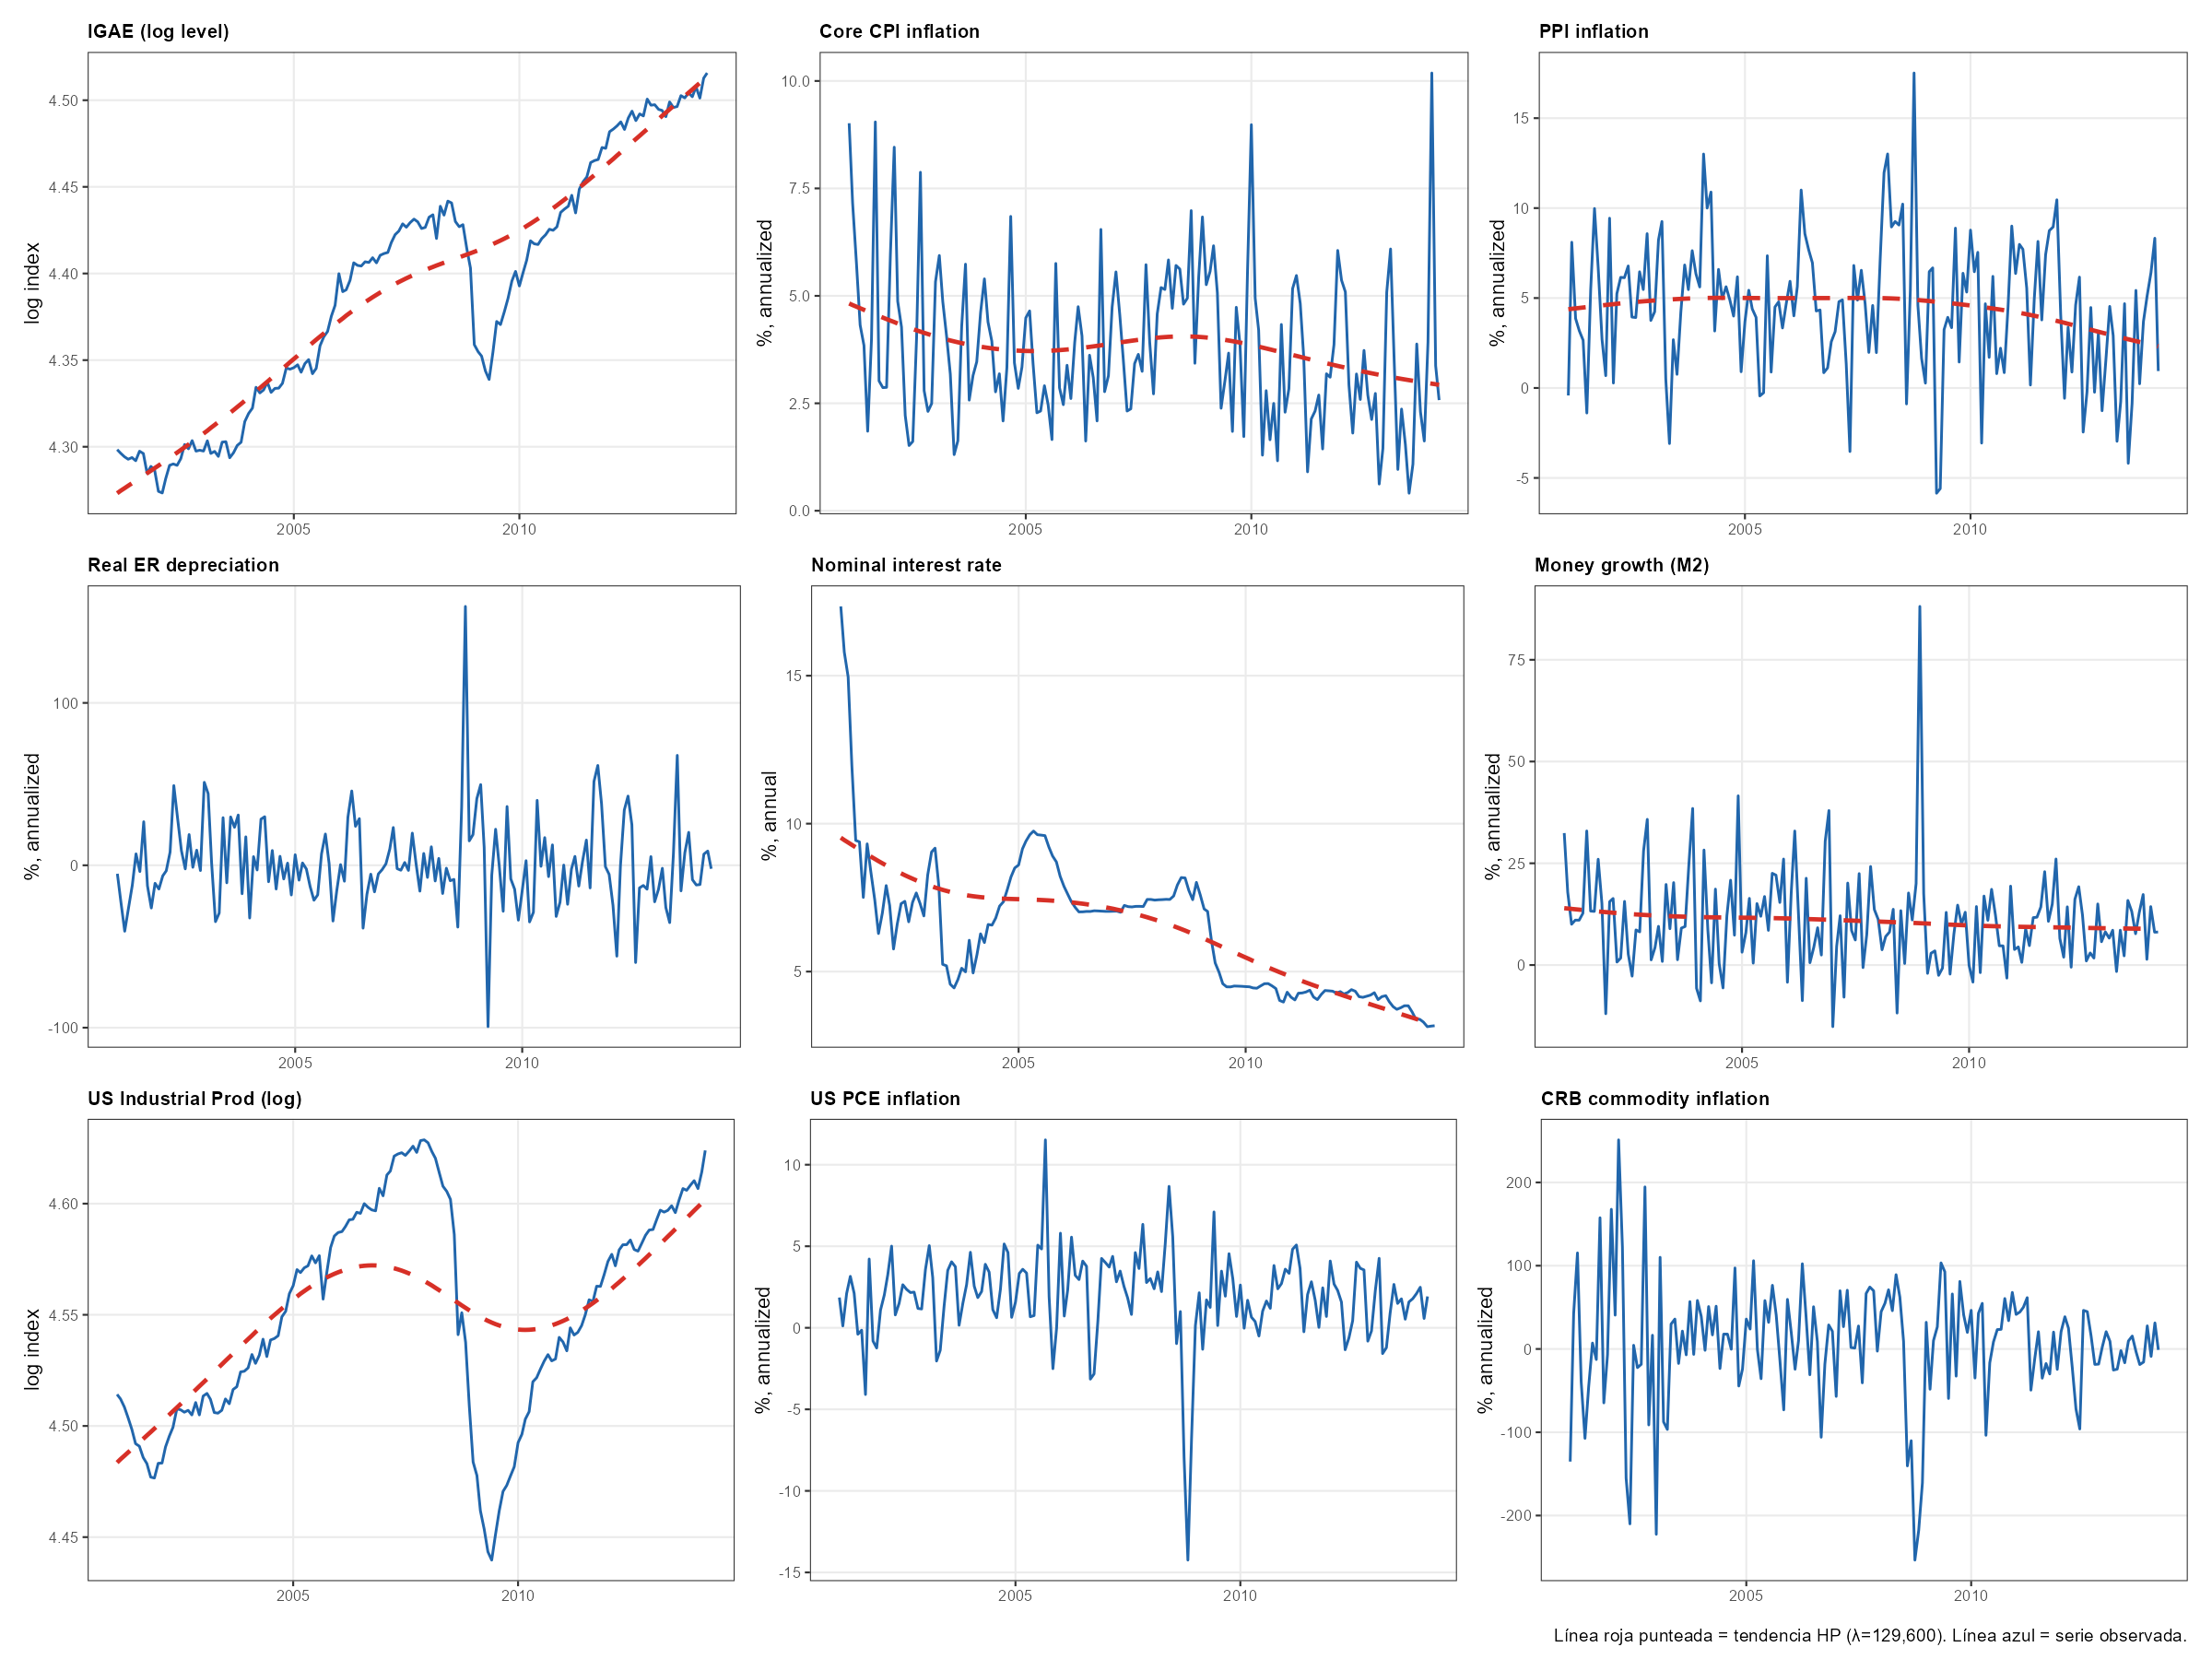
\includegraphics[width=\linewidth]{fig_series_originales.png}
    \caption{Series originales con tendencias HP ($\lambda = 129{,}600$).
    La línea roja punteada indica la tendencia HP; la línea azul es la serie observada.
    El panel inferior reporta las tres variables exógenas del bloque externo.}
    \label{fig:series_originales}
\end{figure}

\begin{figure}[H]
    \centering
    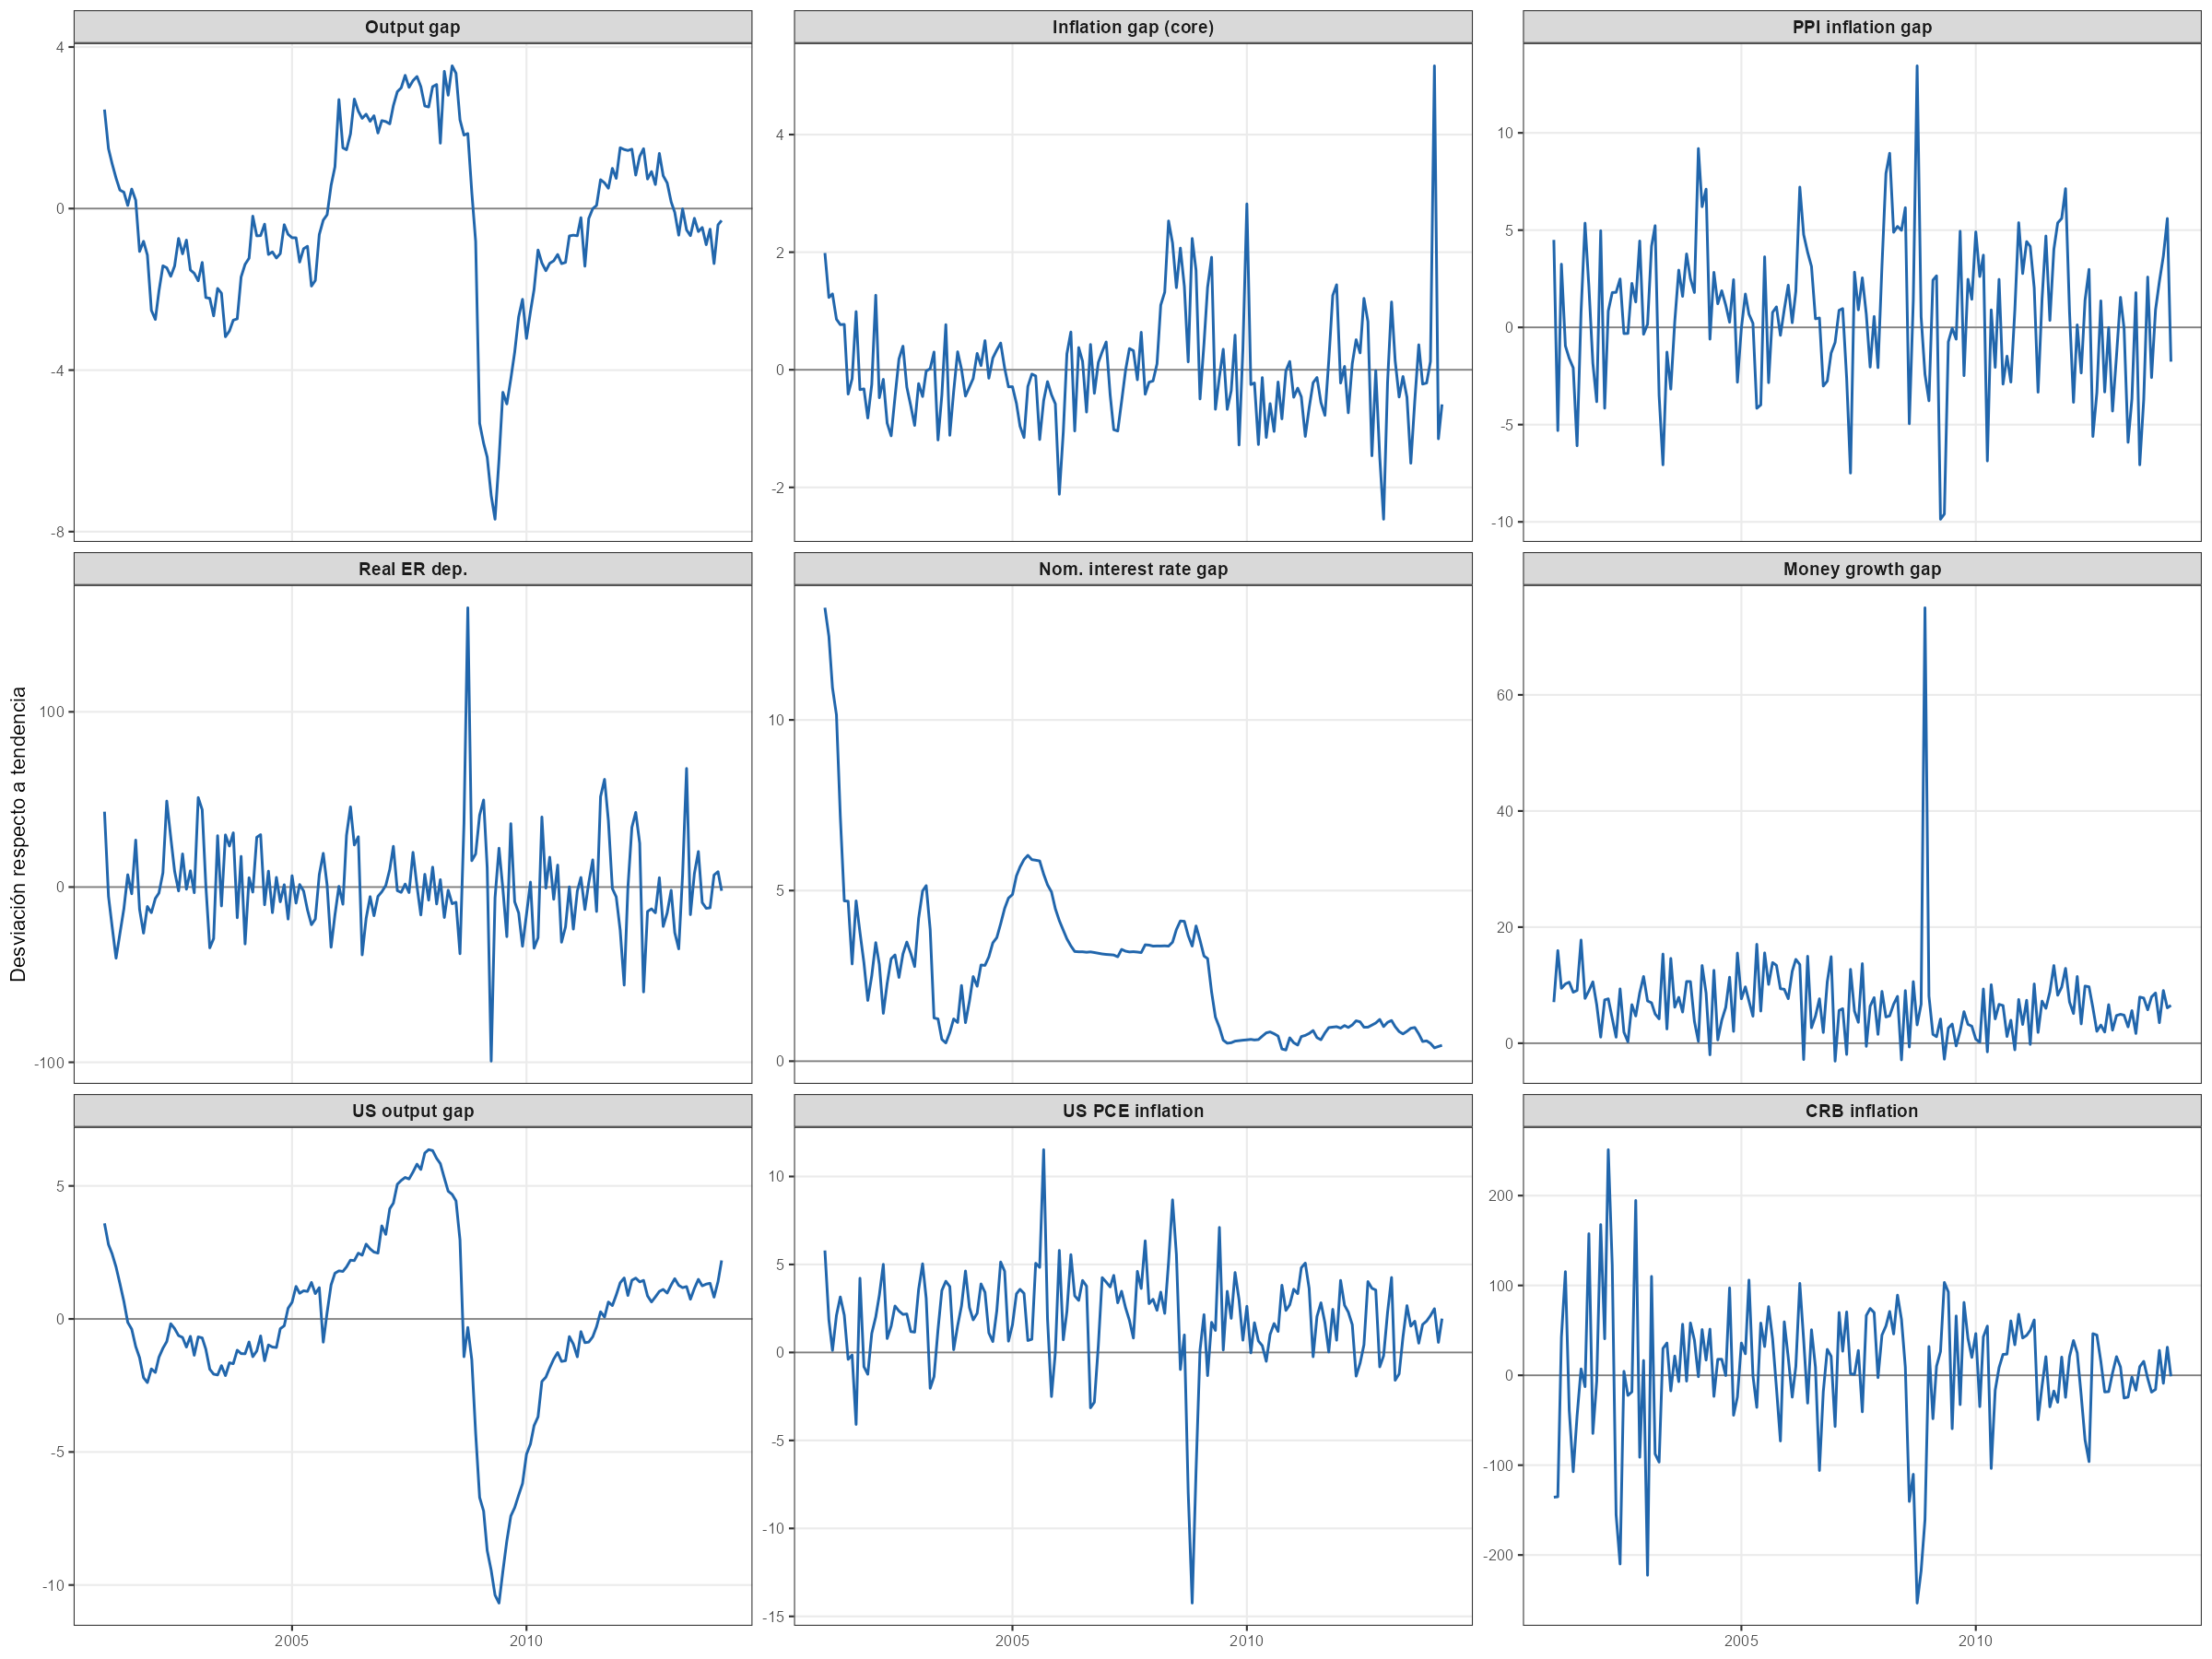
\includegraphics[width=\linewidth]{fig_series_gaps.png}
    \caption{Variables detrended (brechas) utilizadas en la estimación del VAR.
    Equivalente a la Figura 6 de \citet{carrilloelizondo2018}.
    Muestra: enero 2001 -- marzo 2014, $T = 158$.}
    \label{fig:series_gaps}
\end{figure}

Las pruebas de Dickey-Fuller aumentado (ADF) y Phillips-Perron (PP) rechazan la
hipótesis nula de raíz unitaria al 5\% de significancia para todas las series,
consistente con el diseño de las variables como brechas respecto a tendencias
estocásticas (Figura~\ref{fig:adf}).

\begin{figure}[H]
    \centering
    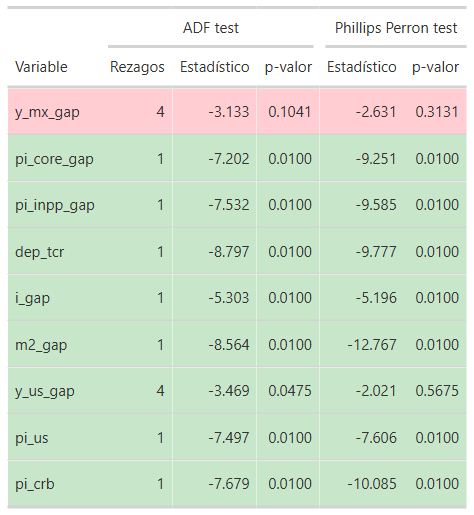
\includegraphics[width=0.95\linewidth]{tabla_adf_pp.png}
    \caption{Pruebas de raíz unitaria ADF y Phillips-Perron.
    Los rezagos ADF se seleccionan con el criterio de Ljung-Box (mínimo $k$ con
    residuos blancos a $p > 0.10$). $H_0$: raíz unitaria.}
    \label{fig:adf}
\end{figure}

La selección del número de rezagos se realiza mediante los criterios de Akaike (AIC),
Schwarz (SIC) y el test de razón de verosimilitud (LR).
El AIC sugiere $p = 2$, el SIC $p = 1$ y el test LR dirime a favor de $p = 3$,
que es el valor adoptado en el paper original (Figura~\ref{fig:varsoc}).
Se sigue la recomendación de \citet{hatemiHacker2009} de usar el LR como criterio de
desempate cuando AIC y SIC difieren.

\begin{figure}[H]
    \centering
    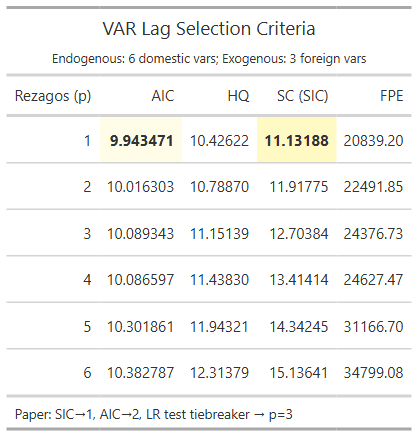
\includegraphics[width=0.75\linewidth]{tabla_varsoc.png}
    \caption{Criterios de selección de rezagos del VAR.
    AIC $\to p=2$; SIC $\to p=1$; test LR $\to p=3$ (decisión final).}
    \label{fig:varsoc}
\end{figure}

% ============================================================
%  4. METODOLOGÍA
% ============================================================
\section{Metodología}
\label{sec:metodologia}

\subsection{Especificación del VAR}

Sea $\Yt = (\text{igae}_t,\, \pi^c_t,\, \pi^p_t,\, \text{dep}_t,\, i_t,\, m_t)'$
el vector de variables endógenas y
$\Zt = (y^{us}_t,\, \pi^{us}_t,\, \pi^{crb}_t)'$
el bloque de variables exógenas.
El VAR(3) de forma reducida se escribe como:
\begin{equation}
    \Yt = \mathbf{c} + \mathbf{A}_1 \Yt_{-1} + \mathbf{A}_2 \Yt_{-2}
         + \mathbf{A}_3 \Yt_{-3} + \mathbf{B}\Zt + \ut,
    \label{eq:var}
\end{equation}
donde $\mathbf{c}$ es un vector de constantes, $\mathbf{A}_j$ son matrices de
coeficientes de dimensión $6 \times 6$, $\mathbf{B}$ es de dimensión $6 \times 3$,
y $\ut \sim \text{i.i.d.}(\mathbf{0},\boldsymbol{\Sigma})$.
El supuesto de bloque exogeneidad implica que $\Zt$ no depende de valores rezagados
de $\Yt$, coherente con la hipótesis de economía pequeña.
Las bandas de incertidumbre se obtienen por el bootstrap de \citet{runkle1987}
con 2,000 réplicas, re-estimando el VAR en cada draw, con intervalos de credibilidad
al 68\% (percentiles 16 y 84).

\subsection{Restricciones de Exclusión (Cholesky)}

La descomposición de Cholesky de la matriz de covarianza $\boldsymbol{\Sigma} = PP'$
identifica el choque monetario como la quinta innovación estructural, correspondiente
a perturbaciones en $i_{\text{gap}}$ ortogonalizadas respecto a igae, $\pi^c$, $\pi^p$
y dep en ese orden.
El ordenamiento lento-rápido implica que el banco central observa el ciclo económico y
la inflación al fijar la tasa en el período corriente, pero el producto y los precios
no reaccionan contemporáneamente al choque monetario.
Se estiman dos versiones: el VAR simple (sin variables exógenas) y el VAR con bloque
exógeno, para aislar la contribución de las variables externas.

\subsection{Restricciones de Signo Simples}

El segundo esquema sigue el procedimiento de \citet{uhlig2005}.
En cada iteración del bootstrap, se genera una matriz ortogonal $Q$ aleatoria con la
distribución de Haar sobre el grupo ortogonal $O(6)$, y se forma la candidata
$\mathbf{A}_0 = P_b \cdot Q$, donde $P_b$ es la descomposición de Cholesky de
$\widehat{\boldsymbol{\Sigma}}$ en la replicación $b$.
El choque monetario corresponde a la quinta columna de $\mathbf{A}_0$.
Un modelo $Q$ es aceptado si la respuesta contemporánea satisface las restricciones de
signo de la Tabla~\ref{tab:sign_restr}.
El proceso se repite hasta reunir $K = 100$ modelos aceptados por draw bootstrap,
con un máximo de $K_{\max} = 5{,}000$ candidatos por draw.

\begin{table}[H]
    \centering
    \caption{Restricciones de signo sobre la respuesta al impacto ($h=0$)
    ante un choque monetario contractivo. Reproducción de la Tabla 2 de
    \citet{carrilloelizondo2018}.}
    \label{tab:sign_restr}
    \begin{tabular}{lcc}
        \toprule
        Variable & Símbolo & Restricción \\
        \midrule
        Brecha del producto    & igae          & $-$ \\
        Inflación subyacente   & $\pi^c$       & $-$ \\
        Inflación al productor & $\pi^p$       & libre \\
        Depreciación TCR       & dep           & $-$ \\
        Tasa de interés        & $i_{\text{gap}}$ & $+$ \\
        Crecimiento M2         & $m_{\text{gap}}$ & $-$ \\
        \bottomrule
    \end{tabular}
\end{table}

\subsection{Restricciones de Signo Aumentadas}

El tercer esquema incorpora una restricción adicional sobre la magnitud de la
respuesta contemporánea de la inflación, siguiendo a \citet{carrilloelizondo2018}.
Se estima la regresión:
\begin{equation}
    \Delta\pi_t = \beta_0 + \beta_i \Delta i_t
                + \beta_{ii} D_t \Delta i_t + \omega_t,
    \label{eq:beta}
\end{equation}
donde $D_t = \mathbf{1}[\Delta i_t \cdot \Delta\pi_t < 0]$ indica períodos en que
la tasa y la inflación se mueven en direcciones opuestas, y $\omega_t$ sigue un proceso
ARMA(1,2) que justifica la corrección de Newey-West con $l = 3$ rezagos.
El coeficiente de interés $\beta_i$ se estima por Mínimos Cuadrados Ordinarios con
corrección HAC de \citet{neweywest1987}, produciendo
$\hat{\beta}^- \approx -0.401$ (SE $\approx 0.194$).
La cota inferior al 95\% de confianza es:
\begin{equation}
    \blower = \hat{\beta}^- - 1.645 \times \text{SE} \approx -0.721,
    \label{eq:blower}
\end{equation}
muy próxima al valor de $-0.700$ reportado por \citet{carrilloelizondo2018}.
Solo se aceptan modelos $Q$ donde $\blower \cdot \Delta i \leq \Delta\pi \leq 0$:
la inflación debe caer al impacto, pero no más de lo que la evidencia histórica permite.

% ============================================================
%  5. RESULTADOS
% ============================================================
\section{Resultados}
\label{sec:resultados}

\subsection{Diagnósticos del VAR}

El VAR(3) estimado satisface los requisitos de estabilidad: todas las raíces del
polinomio característico se encuentran dentro del círculo unitario
(Figura~\ref{fig:varstable}), garantizando que el sistema es estacionario e invertible.
El test de Portmanteau (Ljung-Box) sobre los residuos del sistema no rechaza la hipótesis
nula de no autocorrelación para la mayoría de los rezagos evaluados
(Figura~\ref{fig:lm}), con la excepción de la ecuación de la brecha del producto para
rezagos pequeños, resultado que el paper original también documenta y que justifica
mantener $p = 3$.

\begin{figure}[H]
    \centering
    \begin{subfigure}[b]{0.45\linewidth}
        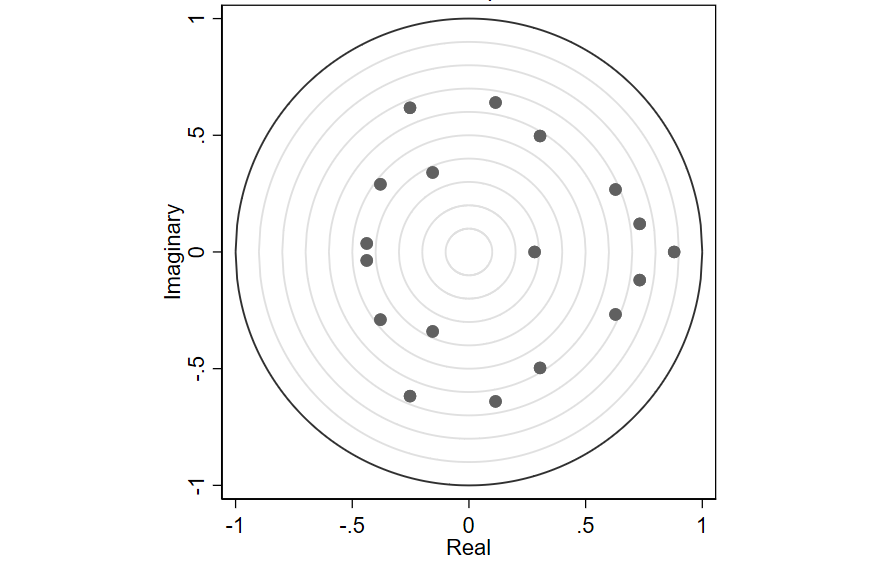
\includegraphics[width=\linewidth]{varstable.png}
        \caption{Raíces del polinomio característico.
        Todas dentro del círculo unitario.}
        \label{fig:varstable}
    \end{subfigure}
    \hfill
    \begin{subfigure}[b]{0.52\linewidth}
        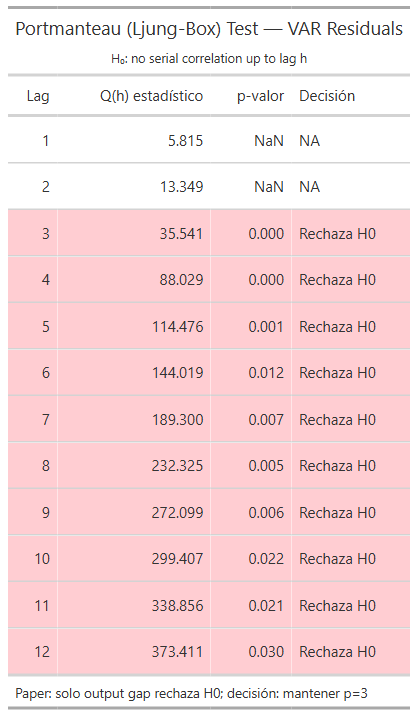
\includegraphics[width=\linewidth]{tabla_lm_norm.png}
        \caption{Test de Portmanteau (Ljung-Box) sobre residuos del VAR(3).
        $H_0$: no autocorrelación hasta el rezago $h$.}
        \label{fig:lm}
    \end{subfigure}
    \caption{Diagnósticos del VAR(3).}
\end{figure}

\subsection{Restricciones de Exclusión (Figura~\ref{fig:fig7})}

La Figura~\ref{fig:fig7} presenta las funciones de impulso-respuesta ante un choque
monetario contractivo bajo el esquema Cholesky, para el VAR simple y el VAR con bloque
exógeno, con bandas de credibilidad al 68\%.
En el VAR simple, la respuesta del producto es débil e imprecisa en los primeros meses,
con un episodio de \textit{price puzzle} leve: la inflación tiende a subir en el
impacto antes de corregirse, patrón que el paper original también reporta.
Bajo el VAR con exógenas, la brecha del producto cae gradualmente hasta un mínimo
alrededor del décimo mes, y la inflación subyacente exhibe un patrón hump-shaped
con pico alrededor del sexto mes antes de caer.
La inclusión de las variables externas resulta, por tanto, cuantitativamente importante:
reduce la probabilidad del \textit{price puzzle} y acota las bandas de credibilidad
para la respuesta del producto, confirmando el papel de las variables de información
forward-looking destacado por \citet{eichenbaum1992} y \citet{hanson2004}.

\begin{figure}[H]
    \centering
    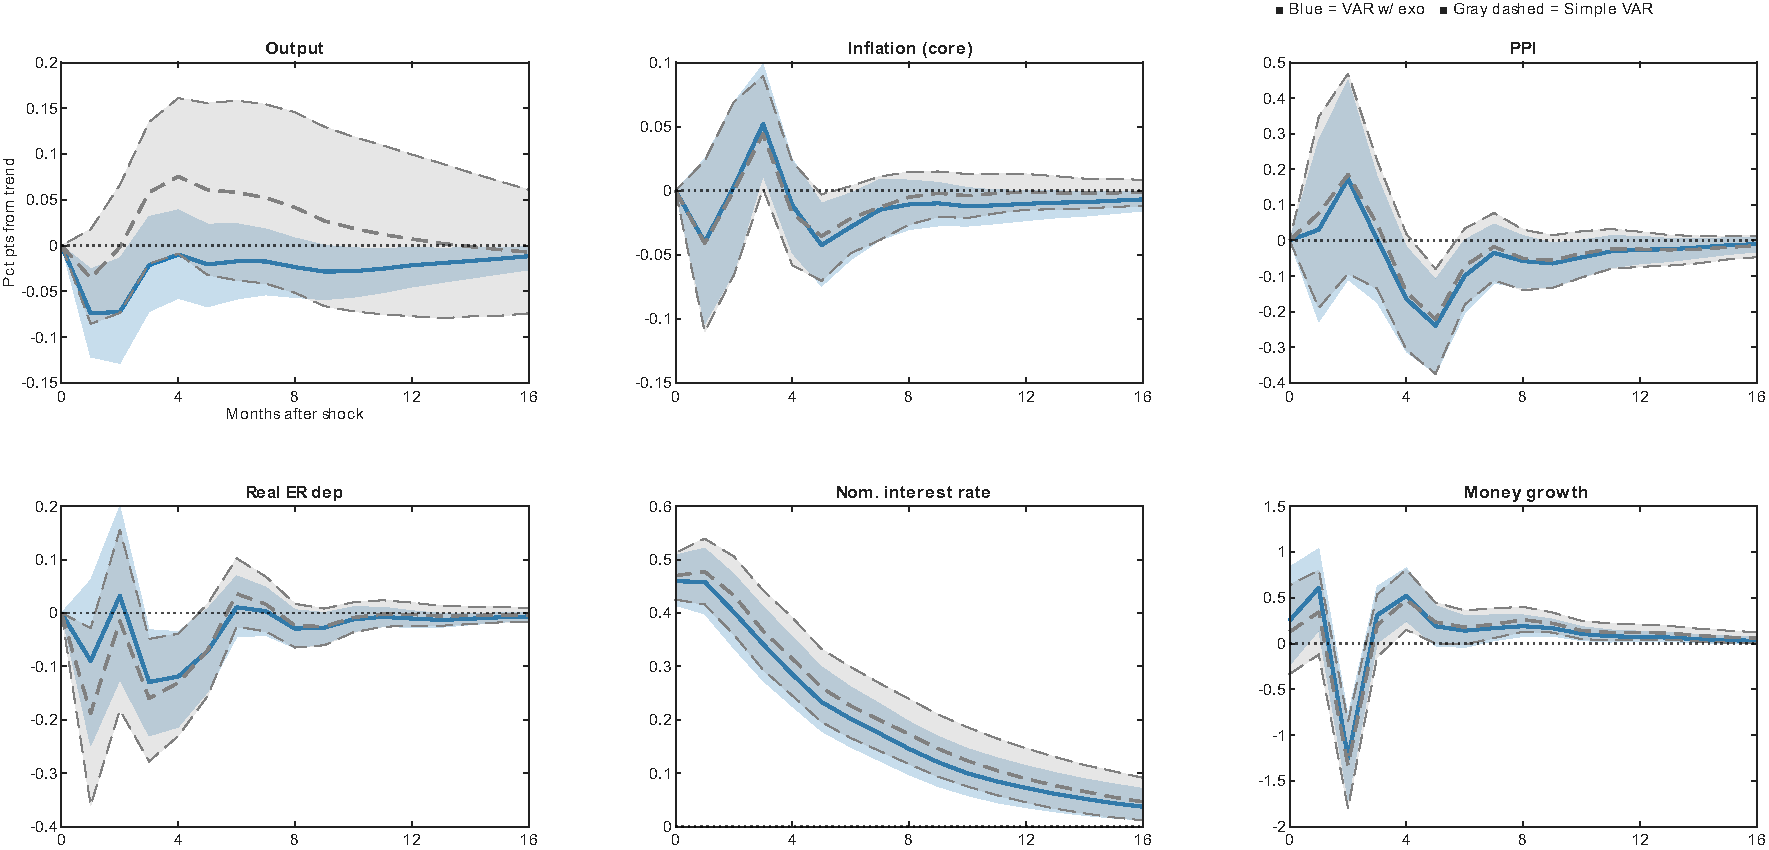
\includegraphics[width=\linewidth]{fig7_exclusion.pdf}
    \caption{Funciones de impulso-respuesta: restricciones de exclusión (Cholesky).
    Fila superior: VAR simple. Fila inferior: VAR con bloque exógeno.
    Banda sombreada: intervalo de credibilidad al 68\% (bootstrap Runkle 1987,
    2{,}000 réplicas). Equivalente a la Figura 7 de \citet{carrilloelizondo2018}.}
    \label{fig:fig7}
\end{figure}

\subsection{Restricciones de Signo Simples y Aumentadas (Figura~\ref{fig:fig8})}

La Figura~\ref{fig:fig8} reporta las medianas de las funciones de impulso-respuesta
bajo las cuatro variantes de restricciones de signo: estándar y aumentada, con y sin
bloque exógeno.
El contraste más notable se observa en la respuesta contemporánea de la inflación
subyacente.
Bajo restricciones simples, la inflación cae en el impacto aproximadamente
$-0.226$ puntos porcentuales anualizados, una magnitud considerablemente mayor a la
sugerida por la elasticidad histórica $\pi$-$i$.
Este resultado refleja el problema de multiplicidad propio de las restricciones de
signo: el espacio de modelos admisibles incluye especificaciones con elasticidades
implausiblemente grandes, y la mediana del conjunto acepta esas respuestas extremas.

Bajo restricciones aumentadas, la cota $\blower = -0.721$ elimina los modelos con
respuestas excesivas, y la inflación de impacto se reduce a $-0.064$ puntos
porcentuales, un resultado que el propio \citet{carrilloelizondo2018} interpreta como
más consistente con la evidencia microeconómica sobre la rigidez nominal de precios.
Esta es la contribución central del esquema de restricciones aumentadas: proporcionar
identificación más informativa sin imponer supuestos cualitativos adicionales.

\begin{figure}[H]
    \centering
    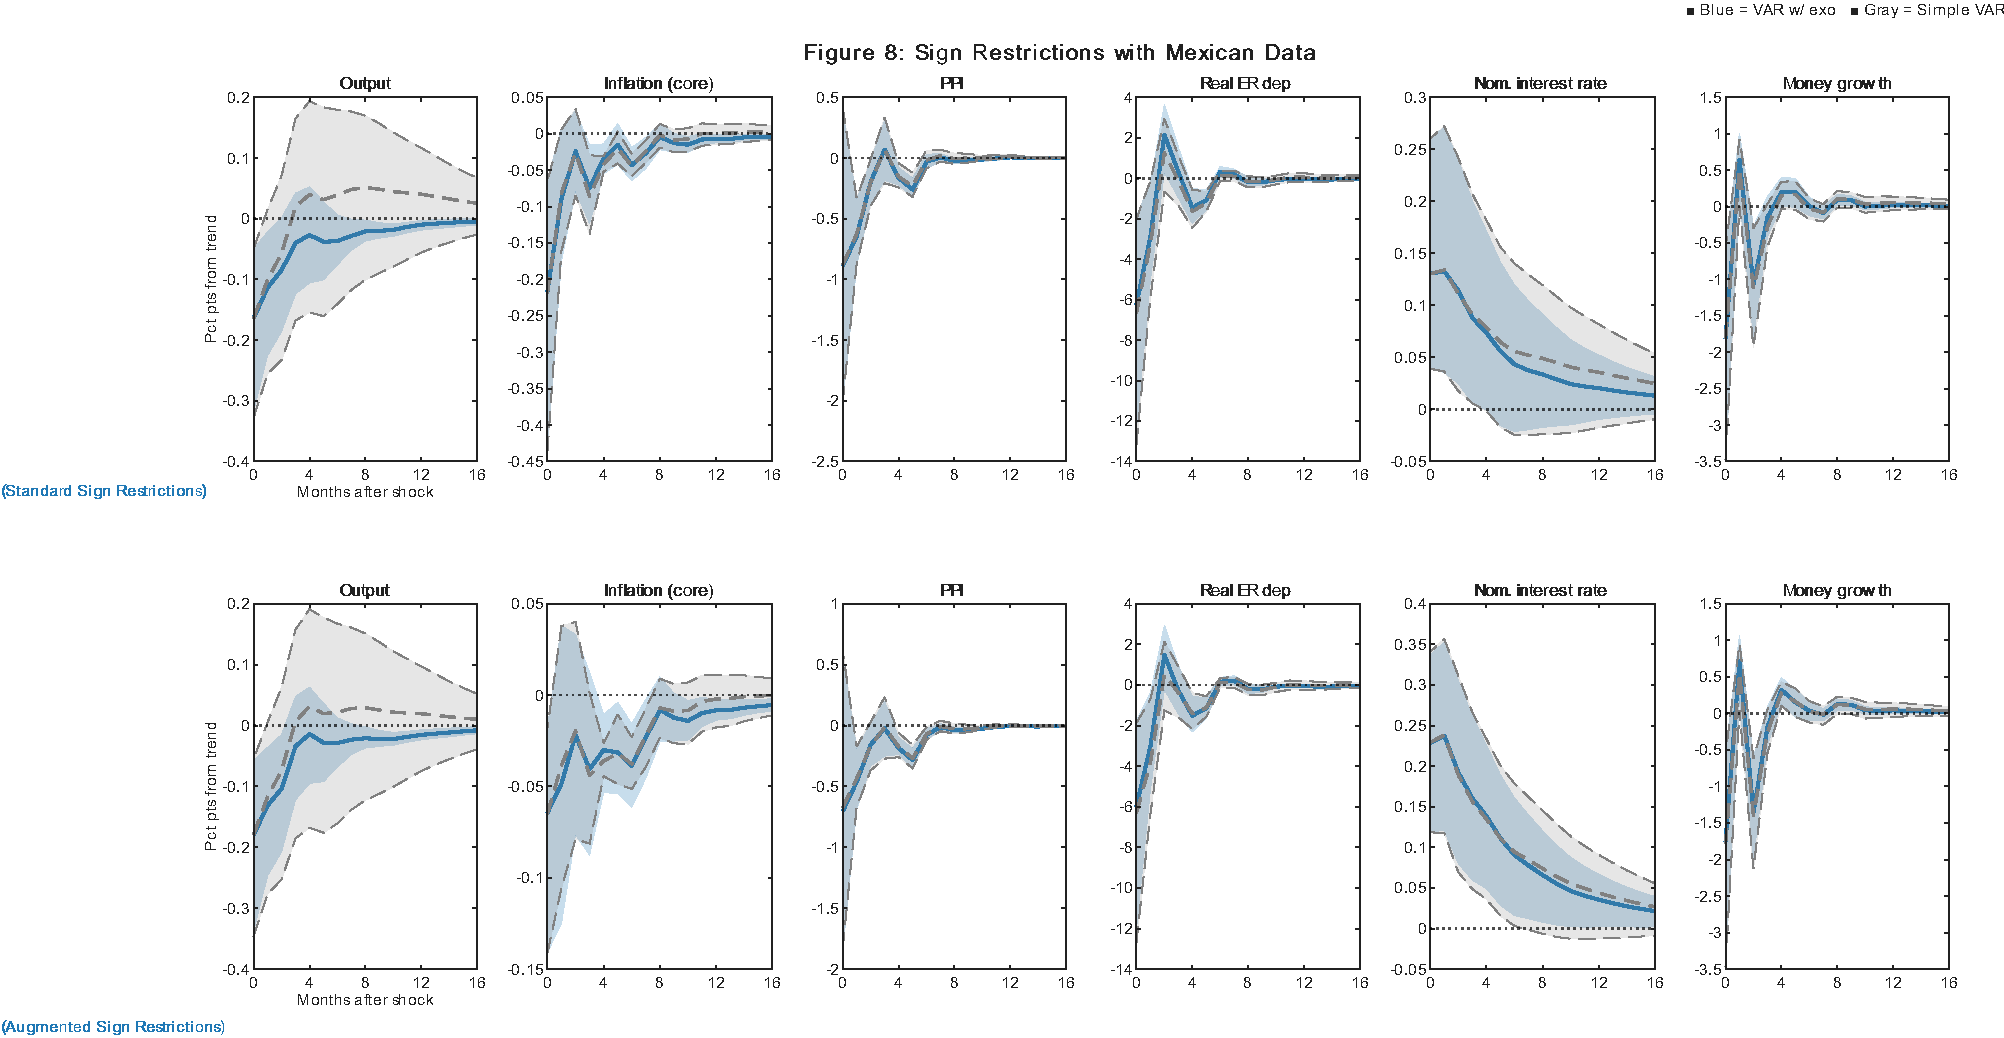
\includegraphics[width=\linewidth]{fig8_sign_restrictions.pdf}
    \caption{Funciones de impulso-respuesta: restricciones de signo.
    Filas superiores: restricciones simples (izquierda: sin exógenas;
    derecha: con exógenas). Filas inferiores: restricciones aumentadas.
    La mediana se traza sobre $K = 100$ modelos aceptados por draw bootstrap
    (2{,}000 draws). $\blower = -0.721$.
    Equivalente a la Figura 8 de \citet{carrilloelizondo2018}.}
    \label{fig:fig8}
\end{figure}

\subsection{Comparación entre Estrategias (Figura~\ref{fig:fig9})}

La Figura~\ref{fig:fig9} superpone las funciones de impulso-respuesta de las tres
estrategias de identificación para el VAR con exógenas.
En el panel superior se comparan Cholesky y restricciones aumentadas; en el panel
inferior, restricciones simples y aumentadas.
Varias regularidades emergen de este ejercicio comparativo.

Primera, las tres estrategias convergen cualitativamente en horizontes de seis a doce
meses: un choque monetario contractivo reduce el producto, la inflación subyacente y
el crecimiento de M2, aprecia el tipo de cambio real, y la tasa de interés vuelve
gradualmente a su nivel de largo plazo conforme el choque se disipa.
Esta convergencia constituye la evidencia de robustez cualitativa que el paper original
destaca.

Segunda, la diferencia entre esquemas de identificación es cuantitativamente más
pronunciada en el corto plazo, particularmente en la respuesta de impacto de la
inflación.
Las restricciones de signo simples producen efectos contemporáneos de inflación hasta
tres veces mayores que las restricciones aumentadas, mientras que Cholesky, por
construcción, impone que la inflación no reacciona en el período de impacto (respuesta
nula exacta).

Tercera, la respuesta del tipo de cambio real es más pronunciada bajo restricciones de
signo en el corto plazo, sugiriendo que el espacio de modelos admisibles incluye
especificaciones con un fuerte canal de tipo de cambio en el período contemporáneo.

\begin{figure}[H]
    \centering
    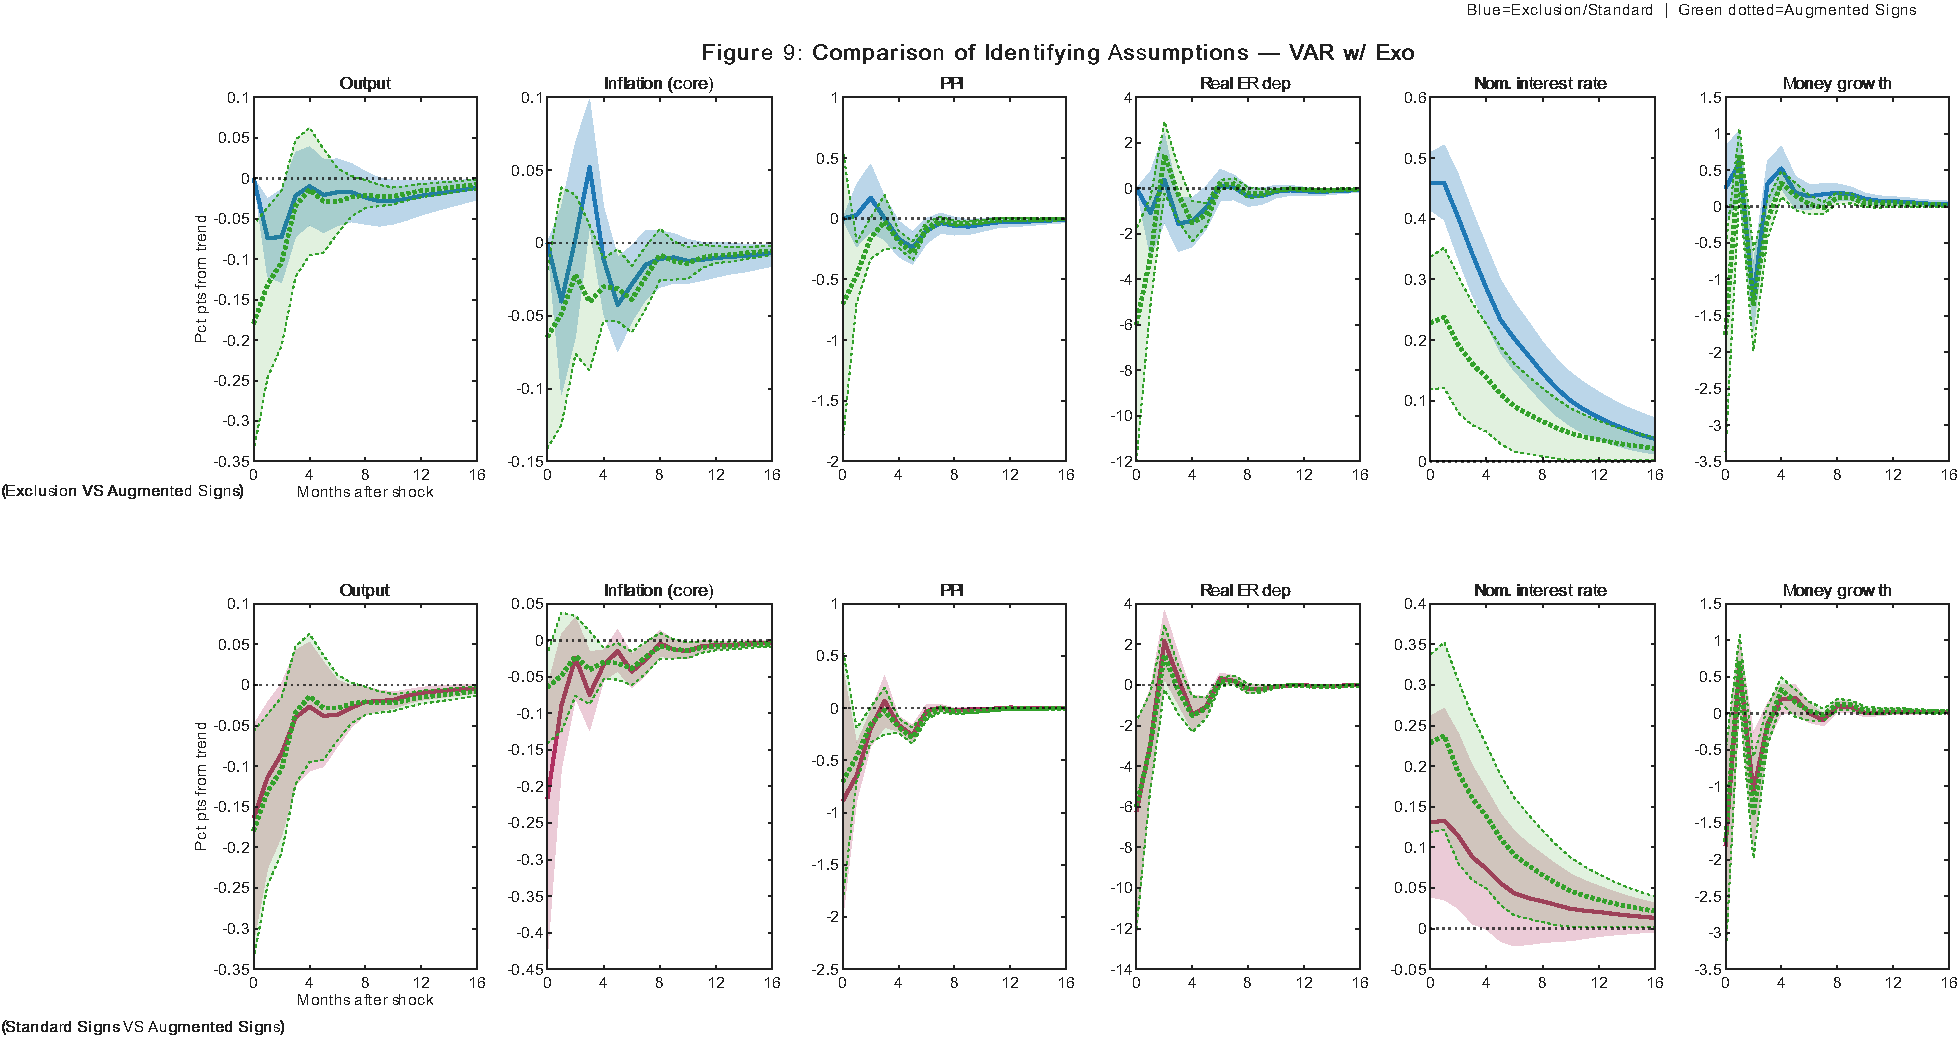
\includegraphics[width=\linewidth]{fig9_comparison.pdf}
    \caption{Comparación de funciones de impulso-respuesta entre estrategias de
    identificación. Panel superior: Cholesky (línea sólida azul) vs.\ restricciones
    aumentadas (línea punteada verde). Panel inferior: restricciones simples (magenta)
    vs.\ restricciones aumentadas (verde). VAR con bloque exógeno.
    Equivalente a la Figura 9 de \citet{carrilloelizondo2018}.}
    \label{fig:fig9}
\end{figure}

\subsection{Resumen Cuantitativo}

La Tabla~\ref{tab:impact} sintetiza las respuestas al impacto ($h = 0$) ante un choque
monetario contractivo de una desviación estándar bajo los tres esquemas, para el VAR
con exógenas.

\begin{table}[H]
    \centering
    \caption{Respuestas al impacto ($h = 0$): comparación entre estrategias de
    identificación. VAR con bloque exógeno.
    Choque: incremento de una desviación estándar en $i_{\text{gap}}$.}
    \label{tab:impact}
    \begin{tabular}{lccc}
        \toprule
        Variable & Cholesky & Sign. simples & Sign. aumentadas \\
        \midrule
        Brecha del producto    & $0.000^*$ & $-0.170$ & $-0.183$ \\
        Inflación subyacente   & $0.000^*$ & $-0.226$ & $-0.064$ \\
        Inflación al productor & $0.000^*$ & $-0.954$ & $-0.797$ \\
        Depreciación TCR       & $0.000^*$ & $-6.326$ & $-6.071$ \\
        Tasa de interés        & $+0.466$  & $+0.129$ & $+0.228$ \\
        Crecimiento M2         & $+0.313$  & $-1.961$ & $-1.897$ \\
        \bottomrule
        \multicolumn{4}{l}{\footnotesize $^*$ Cero por construcción del ordenamiento Cholesky.}\\
        \multicolumn{4}{l}{\footnotesize Sign.\ simples y aumentadas: mediana de modelos aceptados.}\\
    \end{tabular}
\end{table}

% ============================================================
%  6. CONCLUSIONES
% ============================================================
\section{Conclusiones}
\label{sec:conclusiones}

Este trabajo replicó el ejercicio empírico de \citet{carrilloelizondo2018} para México
y evaluó la robustez de las conclusiones sobre política monetaria ante tres estrategias
de identificación en el SVAR.
Los resultados confirman el hallazgo central del paper original: las tres estrategias
convergen cualitativamente en su descripción de la transmisión monetaria para horizontes
de seis a doce meses.
Un choque contractivo reduce el producto y la inflación, aprecia el tipo de cambio real
y contrae los agregados monetarios, con efectos que se materializan gradualmente.

La principal diferencia entre esquemas se concentra en la respuesta contemporánea de la
inflación.
Las restricciones de signo simples generan efectos de impacto implausiblemente grandes
al aceptar modelos con elasticidades inflación-tasa que la evidencia histórica no
respalda.
Las restricciones aumentadas corrigen esta debilidad sin imponer ceros adicionales,
acotando la respuesta contemporánea a valores coherentes con la elasticidad estimada
$\blower \approx -0.721$ —prácticamente idéntica al valor de $-0.700$ del paper
original.
Este resultado es la justificación central del esquema de restricciones aumentadas
propuesto por \citet{carrilloelizondo2018}: proporciona mayor contenido informativo
que las restricciones de signo simples sin la arbitrariedad implícita en las
restricciones de exclusión.

\eliminar{Revisar si esta sección de conclusiones es suficientemente larga o si el profesor espera mayor discusión de implicaciones de política monetaria.}
Quedan fuera del alcance de este trabajo varias extensiones.
El análisis asume linealidad y parámetros constantes en el tiempo, supuesto que podría
cuestionarse ante el episodio de la crisis de 2008-2009, que cae dentro de la muestra.
Adicionalmente, las diferencias de fuente en el tipo de cambio real y en el método de
ajuste estacional introducen discrepancias menores no eliminables.
Trabajos futuros podrían explorar la robustez de los resultados bajo especificaciones con
cambio de régimen o con datos de mayor frecuencia que mejor capturen la dinámica de
corto plazo de la transmisión monetaria en México.

% ============================================================
%  BIBLIOGRAFÍA
% ============================================================
\bibliography{references}

\end{document}
